\documentclass{article}[jsarticle]
\usepackage[T1]{fontenc}
\usepackage[dvipdfmx]{hyperref}
\usepackage{lmodern}
\usepackage{latexsym}
\usepackage{amsfonts}
\usepackage{amssymb}
\usepackage{mathtools}
\usepackage{nccmath}
\usepackage{amsthm}
\usepackage{multirow}
\usepackage[dvipdfmx]{graphicx}
\usepackage{wrapfig}
\usepackage{here}
\usepackage{float}
\usepackage{ascmac}
\usepackage{url}

\title{数理科学概論 課題2}
\author{高林秀 \\ 三宅研究室 博士前期課程1年 \\ V-CampusID : 23vr008n}
\date{\today}

\begin{document}

\maketitle

\setcounter{section}{-1}

\section{問題概要}
本課題の問題は以下1~3の内容である。以降の章でそれぞれについて解答するものとする。

\begin{enumerate}
    \item クロスエントロピーが計算可能であるためには、モデルの出力$\hat{y}$の値はある範囲内でなければならない。
    クロスエントロピーの式からその範囲がどのようになるか、説明せよ。

    \item 以下の表には、5つのデータからなる2値分類問題で、case 1~6 の6つの場合において、モデル出力がまとめられている。
    それぞれのケースについて、5つのデータのクロスエントロピーの平均値を求めよ。\par 
    また、各ケースの二乗平均誤差 (モデル出力と正解ラベルの差の二乗の平均値) も求めよ。
    \begin{figure}[H]
        \centering
        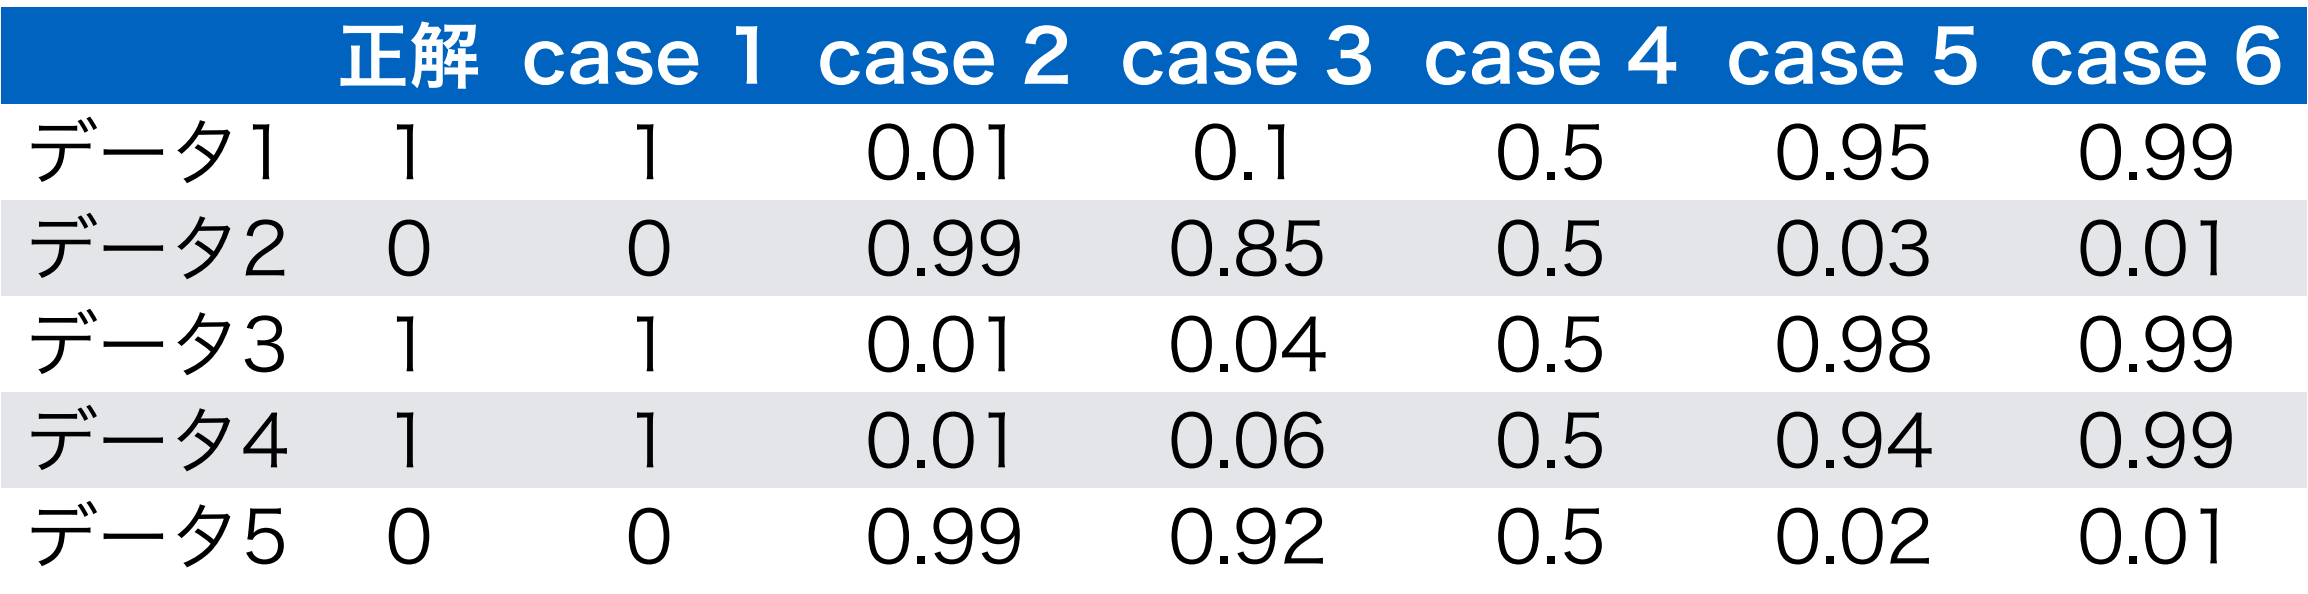
\includegraphics[scale=0.3]{./2023-06-23215207.png}
    \end{figure}

    \item クロスエントロピーと二乗平均誤差について、(2) で計算した値からわかる範囲で共通点と相違点について考察せよ。
    ただし、各ケースでの値を直接比較するのではなく、ケースの変化に対して値がどのように変化していくかについて考察すること。
    
\end{enumerate}

\subsection{制約条件}
この問題で求めるクロスエントロピーは、対数の底を $e$ としたものとすること。$0\log_{e}0$は数学においては本来計算不可能な量だが、
本問題においてもし出てきた場合には0としてよいものとする。


\section{問1} 
\subsection{問題文}
クロスエントロピーが計算可能であるためには、モデルの出力$\hat{y}$の値はある範囲内でなければならない。クロスエントロピーの式からその範囲がどのようになるか、説明せよ。
\subsection{解答}
結論から言えば、クロスエントロピーが計算可能であるためにはモデルの出力$\hat{y}$の値の範囲は、$0 < \hat{y} < 1$である必要がある。\par 
これは、クロスエントロピーの式とグラフを考えることで分かる。クロスエントロピーの式は以下のようになる。
\begin{equation}
    H(q, p) = -\sum_{x}q(x)\log_{e}p(x)\\
    \text{ここで、}q(x) = \text{正解ラベルの確率分布}p(x) = \text{予測値の確率分布} = \hat{y}
\end{equation}
分類問題において、クロスエントロピー誤差関数は、予測確率$p(x)$と正解ラベル$q(x)$の間の距離、不一致度を表す。
このとき、$q(x)$は、正解ラベルのみが1でそれ以外が0であるような確率分布であり、これはone-hotエンコーディングと呼ばれる。\par
ゆえに、ラベルの予測確率$p(x)$のみが誤差関数に影響を与えるので、分類問題ではクロスエントロピー誤差関数は、以下のような式になる。
\begin{equation}
    -\log_{e}p(x)
\end{equation}
このとき、クロスエントロピーのグラフは以下のようになる。
\begin{figure}[H]
    \centering
    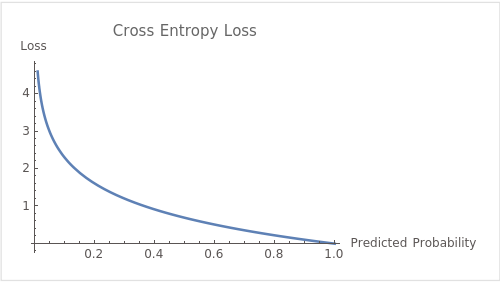
\includegraphics[scale=0.5]{./0ede6696-cbe7-4a39-b001-95edbb54e133.png}
\end{figure}
このグラフから、$p(x)$の値が0に近づくにつれて、その極限は無限大に発散していくことが分かる。従って、$p(x)$の値が0になることは許されない。
また、$p(x)$の値が1に近づくにつれて、その極限は0に収束していくことが分かる。クロスエントロピーの式から、$-\log_{e} 0 = \infty$であるため、
$p(x)$の値が1になることも許されない。\par
ゆえに、モデルの出力$\hat{y}$の値の範囲は、$0 < \hat{y} < 1$である必要がある。


\section{問2}
\subsection{問題文}
以下の表には、5つのデータからなる2値分類問題で、case 1~6 の6つの場合において、モデル出力がまとめられている。
それぞれのケースについて、5つのデータのクロスエントロピーの平均値を求めよ。\par 
また、各ケースの二乗平均誤差 (モデル出力と正解ラベルの差の二乗の平均値) も求めよ。
\begin{figure}[H]
    \centering
    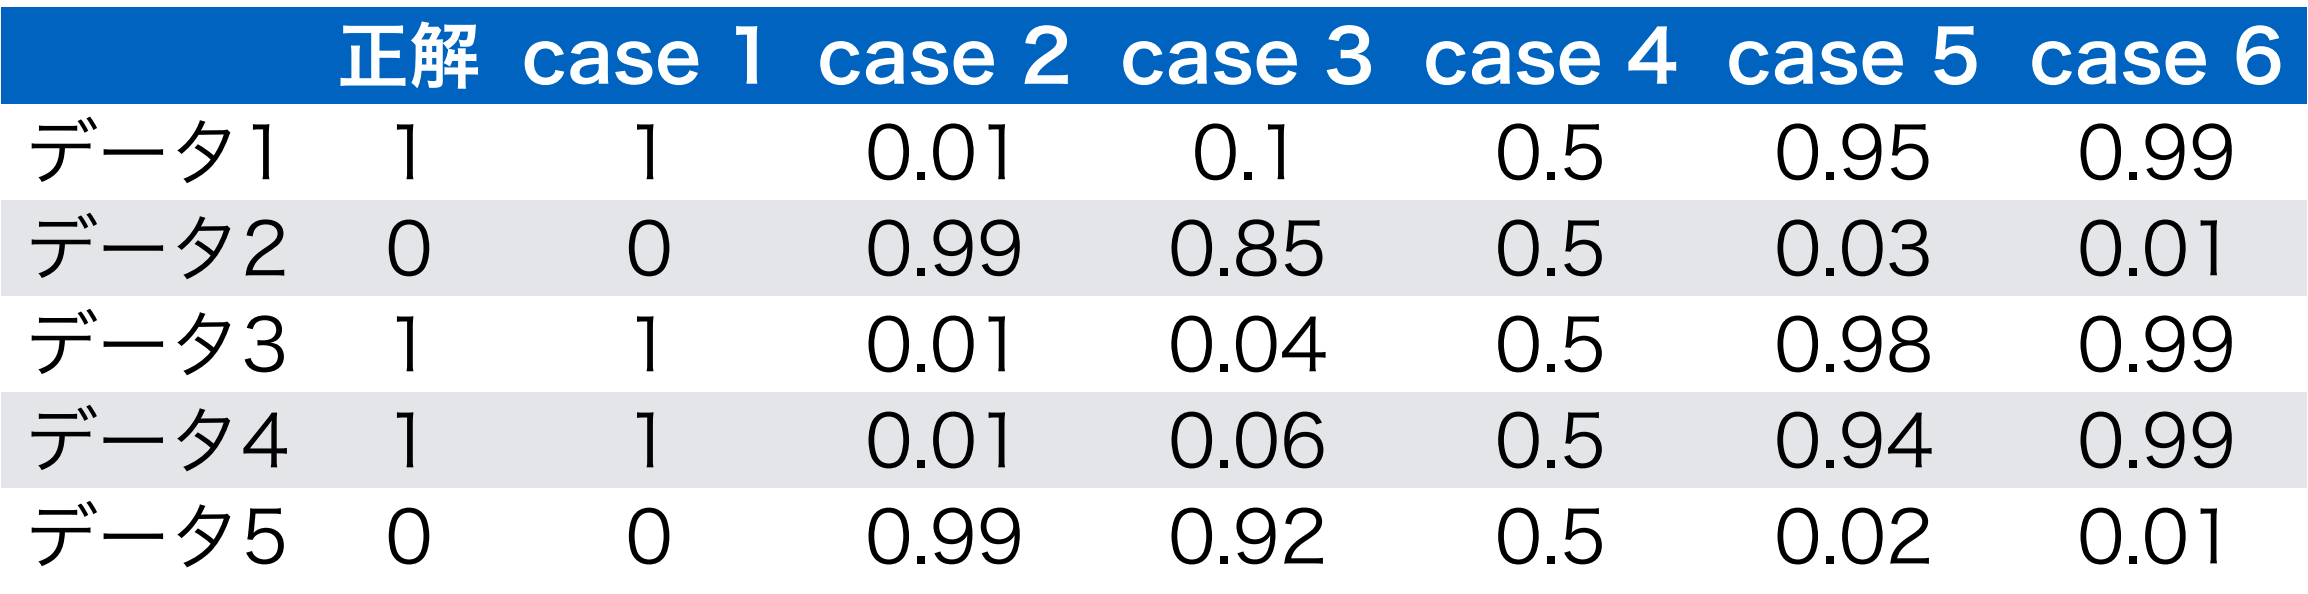
\includegraphics[scale=0.3]{./2023-06-23215207.png}
\end{figure}
\subsection{解答}
まず各データの、それぞれのケース毎にクロスエントロピーを計算した結果を以下に示す。なお計算は、巻末付録に付属のPythonコードを用いて行った。
過程を参照する際は、そちらを参照されたい。
\begin{table}[H]
    \begin{tabular}{lc|c|c|c|c|c|c}
          & 正解 & case1 & case2 & case3 & case4 & case5 & case6 \\
    data1 & 1  & 0     & 4.60  & 2.30  & 0.69  & 0.05  & 0.01  \\
    data2 & 0  & 0     & 4.60  & 1.89  & 0.69  & 0.03  & 0.01  \\
    data3 & 1  & 0     & 4.60  & 3.21  & 0.69  & 3.50  & 4.60  \\
    data4 & 1  & 0     & 4.60  & 2.81  & 0.69  & 0.06  & 0.01  \\
    data5 & 0  & 0     & 4.60  & 2.52  & 0.69  & 0.02  & 0.01 
    \end{tabular}
    \end{table}
このデータから、各ケース毎のクロスエントロピーの平均値を以下に示す。
\begin{itemize}
    %\caption{クロスエントロピーの平均値}
    \item case1 : 0 (正確には計算不能)
    \item case2 : 4.60
    \item case3 : 2.55
    \item case4 : 0.69
    \item case5 : 0.73
    \item case6 : 0.92
\end{itemize}
また、各ケース毎の二乗平均誤差(MSE)を以下に示す。
\begin{itemize}
    %\caption{二乗平均誤差(MSE)}
    \item case1 : 0.0
    \item case2 : 0.98
    \item case3 : 0.83
    \item case4 : 0.25
    \item case5 : 0.18
    \item case6 : 0.19
\end{itemize}


\section{問3}
\subsection{問題文}
クロスエントロピーと二乗平均誤差について、(2) で計算した値からわかる範囲で共通点と相違点について考察せよ。
ただし、各ケースでの値を直接比較するのではなく、ケースの変化に対して値がどのように変化していくかについて考察すること。
\subsection{解答}
まず、クロスエントロピーと二乗平均誤差はどちらも、機械学習において、正解データとモデルの予測出力の誤差を表す指標として使われる。
前問の各ケース別のクロスエントロピー誤差と、二乗平均誤差の値はそのことを示している。
表の正解ラベルと各caseの出力を比較すればわかるが、モデルの出力と正解ラベルが一致している場合は、両者の誤差値は当然0で、反対に正解とモデルの出力の差が大きい場合、誤差値もそれに付随するように大きくなる。\par
しかし、クロスエントロピーと二乗平均誤差には、以下のような相違点がある。
\begin{itemize}
    \item 分類問題か回帰問題を解くかによって、適切な誤差関数が異なる。
    \item 勾配降下法による学習を行う場合、クロスエントロピーを誤差関数として用いる方が適切である。
    \item 誤差値の意味が両者で異なる。
\end{itemize}
クロスエントロピーは、ロジスティック回帰やニューラルネットワークなど確率的な出力をもつモデルでおける誤差関数として、適している。
ゆえに、今回のような分類問題に関して、そのデータがその程度の確率でどのクラスに属するかを求めるようなモデルにおいては、クロスエントロピーを誤差関数として用いる方が適している。\par 
また、クロスエントロピーは勾配降下法との相性が良いという側面もある。勾配降下法では、微分を用いて関数の勾配、傾きを計算するが、その際クロスエントロピーの式より、微分計算がMSEよりも簡単であるという側面がある。
クロスエントロピーはその式から明らかなように、対数$\log$と自然対数$e$がある。$\log x$の微分形は、$\frac{1}{x}$であり、$e^{x}$の微分形は$e^{x}$である。
微分をしても式が複雑にならないという点において、クロスエントロピーは勾配降下法との相性が良いと言える。\par

また、誤差値の意味においてもMSEとクロスエントロピーでは少し意味が異なる。MSEではその式の通り、誤差の値を2乗しているため、大きな誤差に対して大きな値を返す。
一方、クロスエントロピーもMSE同様誤差が大きければ大きな値をとるが、2乗ではないのに加え、正解とモデルの情報量的な距離を計算するものである。
これは、モデルの正解に対する確信度を表すものであり、MSEとは誤差の意味合いが異なる。\par


\section{付録}
本解答に使用したソースコードは以下のGoogleDriveのリンクから参照できる。
記載形式はJupyter Notebook形式である。
\begin{itemize}
    \item \url{https://drive.google.com/file/d/1MWVYsbSlLHQ2qLyebFIOCXA9AAKX8p5V/view?usp=sharing}
\end{itemize}

\end{document}